% ------------------------------------------------------------------ key highlights at a glance
\begin{frame}{Key highlights at a glance}
    \label{sl:highlights}
    \centering
    \resizebox{\linewidth}{!}{%
    \begin{tikzpicture}[x=3.45cm, y=2.32cm]
        \node[tile=camc] at (0, 0) {{\Large\textbf{\textcolor{camc}{\EfiveFive\ cents}}}\\[3pt]
            \scriptsize camera-only pitch error after 5 taps: \emph{audio teaches vision}\\[2pt]{\tiny slide \pageref{sl:learning}}};
        \node[tile=phyc] at (1, 0) {{\Large\boldmath\textbf{\textcolor{phyc!75!black}{$n = \EthreeN$}}}\\[3pt]
            \scriptsize French's exponent, found by the data (theory: 4)\\[2pt]{\tiny slide \pageref{sl:learning}}};
        \node[tile=micc] at (2, 0) {{\Large\textbf{\textcolor{micc}{\EsixTunedHidden\,\%}}}\\[3pt]
            \scriptsize which of 5 identical bowls rang; striker hidden, 10~dB SNR\\[2pt]{\tiny slide \pageref{sl:results1}}};
        \node[tile=fusc] at (0, -1) {{\Large\textbf{\textcolor{fusc}{\EsixFusedZero{} vs \EsixAudioZero\,\%}}}\\[3pt]
            \scriptsize fused vs audio alone at 0~dB: two clues beat one\\[2pt]{\tiny slide \pageref{sl:results1}}};
        \node[tile=camc] at (1, -1) {{\Large\textbf{\textcolor{camc}{\EsevenIdTap\ cents}}}\\[3pt]
            \scriptsize tuning error for raga Bhupali after one check tap\\[2pt]{\tiny slide \pageref{sl:results2}}};
        \node[tile=gray] at (2, -1) {{\Large\textbf{\textcolor{gray!60!black}{No dataset}}}\\[3pt]
            \scriptsize one physical law, learned from a few taps\\[2pt]{\tiny slide \pageref{sl:physics}}};
    \end{tikzpicture}}
    \vspace{2mm}
    \begin{block}{What I built}
        \scriptsize
        A Python library (audio, vision, physics, fusion, tuning) $\cdot$ a live desktop app (webcam + mic, or simulated)
        $\cdot$ an interactive web explainer with ManimGL animations $\cdot$ experiments E1--E7 and 16 automated tests
        $\cdot$ code: \texttt{github.com/KUSHAGRA2606/TuneSight}
    \end{block}
\end{frame}

% ------------------------------------------------------------------ how it works: the big picture
\begin{frame}{How it works: two senses, one law}
    \label{sl:arch}
    \centering
    \resizebox{\linewidth}{!}{%
    \begin{tikzpicture}[font=\scriptsize, >={Stealth[length=2mm]}, line width=0.6pt,
        box/.style={draw, rounded corners=2pt, align=center, inner sep=3pt, minimum height=10mm, minimum width=20mm},
        cam/.style={box, draw=camc, fill=camc!10}, mic/.style={box, draw=micc, fill=micc!10},
        phy/.style={box, draw=phyc, fill=phyc!12, minimum width=28mm}, fus/.style={box, draw=fusc, fill=fusc!10, minimum width=28mm},
        outbox/.style={box, draw=fusc, fill=fusc!18, minimum height=7mm, minimum width=23mm},
        lab/.style={font=\tiny, inner sep=2.5pt}]
        \foreach \x/\t in {0/sensors, 3.0/what each sense measures, 7.3/reasoning, 11.6/outputs}
            \node[font=\tiny\itshape, text=gray] at (\x, 2.0) {\t};
        \node[cam] (camera) at (0, 1.15) {\textbf{Camera}\\video frames};
        \node[cam] (vision) at (3.0, 1.15) {\textbf{Vision}\\fill of each bowl,\\striker position};
        \node[mic] (micro) at (0, -1.15) {\textbf{Microphone}\\sound};
        \node[mic] (audio) at (3.0, -1.15) {\textbf{Audio}\\strike time,\\pitch};
        \node[phy] (phys) at (7.3, 1.15) {\textbf{The law}\\water level $\to$ pitch\\learned from taps};
        \node[fus] (fusion) at (7.3, -1.15) {\textbf{Fusion}\\sound $\times$ motion clue\\+ ``none of these''};
        \node[outbox] (tune) at (11.6, 1.15) {Tune to a raga};
        \node[outbox] (which) at (11.6, -0.7) {Which bowl?};
        \node[outbox] (sargam) at (11.6, -1.6) {Sargam notation};
        \draw[->, camc] (camera) -- (vision);
        \draw[->, micc] (micro) -- (audio);
        \draw[->, camc] (vision) -- node[lab, above] {fill ratio $r$} (phys);
        \draw[->, micc] (audio) -- node[lab, below] {pitch $f$} (fusion);
        \draw[->, camc, dashed] (vision.south east) -- node[lab, sloped, above, pos=0.45] {striker tip} (fusion.north west);
        \draw[->, phyc] ([xshift=6mm]phys.south) -- node[lab, right, align=left] {predicted pitch\\of every bowl} ([xshift=6mm]fusion.north);
        \draw[->, fusc] ([xshift=-6mm]fusion.north) -- node[lab, left] {learn} ([xshift=-6mm]phys.south);
        \draw[->, phyc] (phys) -- node[lab, above] {water level} (tune);
        \draw[->, fusc] (fusion.east) -- (which.west);
        \draw[->, fusc] (fusion.east) -- (sargam.west);
    \end{tikzpicture}}
    \vspace{1mm}
    \begin{block}{Every strike, in four steps}
        \scriptsize
        \textbf{1. Camera:} how full each bowl is just before the strike, and where the striker tip lands.\\
        \textbf{2. Microphone:} when the strike happened and what pitch it made.\\
        \textbf{3. Fusion:} compare the pitch with every bowl's \emph{predicted} pitch, add the striker clue, pick the bowl.\\
        \textbf{4. Learning:} the tap adds one (fill, pitch) point to the law, so the sound teaches the camera.
    \end{block}
\end{frame}

% ------------------------------------------------------------------ assumptions
\begin{frame}{The assumptions, and why they are reasonable}
    \label{sl:assumptions}
    \scriptsize
    \renewcommand{\arraystretch}{1.12}
    \begin{tabular}{@{}>{\raggedright\arraybackslash}p{0.335\linewidth} >{\raggedright\arraybackslash}p{0.30\linewidth} >{\raggedright\arraybackslash}p{0.30\linewidth}@{}}
        \toprule
        \textbf{Assumption} & \textbf{Why it is reasonable} & \textbf{If it fails} \\
        \midrule
        \textbf{A1.} Bowls are see-through; the water is coloured & the water line is visible by its colour & opaque bowls: look from the top \\
        \textbf{A2.} Same-shape bowls share one law & same glass, same physics \cite{french1983} & one check tap per bowl corrects it \\
        \textbf{A3.} Pitch = lowest strong ring, 150~Hz--8~kHz & the range of glass tumblers & a hum must also start at the strike and fade \\
        \textbf{A4.} One bowl is struck at a time & each sound has one source & needs multi-pitch analysis \\
        \textbf{A5.} The water is read just before the strike & then no hand hides it & use the last clear frames \\
        \textbf{A6.} The camera is fixed; bowls stay in place & each bowl keeps its identity & detect the bowls again \\
        \textbf{A7.} Camera and mic make independent errors & different sensors, different noise & fusion becomes over-confident \\
        \bottomrule
    \end{tabular}
    \vspace{2mm}
    \begin{block}{Why state them}
        \scriptsize
        Each assumption is a place where the system can fail. Naming it tells you what to check in a real setup,
        and it is exactly what the ``scope for improvement'' slide removes, one by one (slide \pageref{sl:improve}).
    \end{block}
\end{frame}

% ------------------------------------------------------------------ hearing
\begin{frame}{Hearing: from a tap to a pitch}
    \label{sl:hearing}
    \centering
    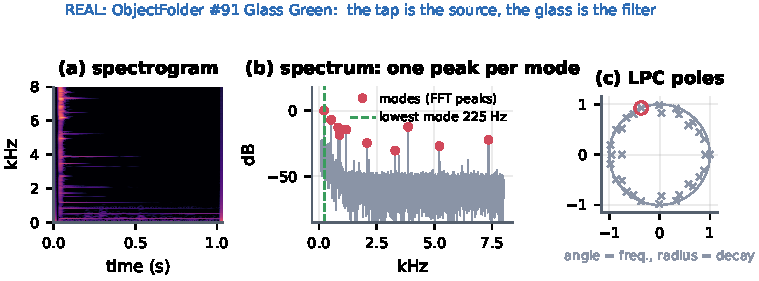
\includegraphics[width=0.80\linewidth]{images/figures/fig_strike.pdf}
    \vspace{-1mm}
    \begin{columns}[T]
    \column{0.47\textwidth}
        \begin{block}{The idea: a source and a filter}
            \scriptsize
            The tap is a short click (the \emph{source}). The bowl rings at a few fixed frequencies, its
            \emph{modes}, each fading like a bell (the \emph{filter}). It is the course's model of speech,
            applied to a bowl. The note we hear is the lowest strong mode.
        \end{block}
    \column{0.51\textwidth}
        \scriptsize
        \textbf{Steps}
        \begin{enumerate}
            \item Find the strike: a sudden jump in loudness.
            \item Spectrum (FFT): each peak is one mode (panel b).
            \item Keep a peak only if it \emph{starts at the strike and fades}: hum and fans are ignored.
            \item Pitch = the lowest strong peak.
            \item Cross-check: a second method (LPC, panel c) must find the same modes.
        \end{enumerate}
    \end{columns}
\end{frame}

% ------------------------------------------------------------------ seeing
\begin{frame}{Seeing: the water level from pixels}
    \label{sl:vision}
    \centering
    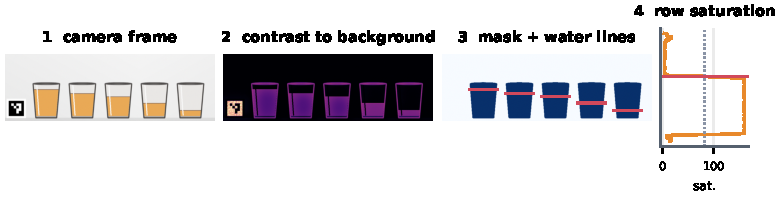
\includegraphics[width=0.96\linewidth]{images/figures/fig_vision_steps.pdf}
    \vspace{-1mm}
    \begin{columns}[T]
    \column{0.52\textwidth}
        \scriptsize
        \textbf{Steps}
        \begin{enumerate}
            \item \textbf{Background:} smooth away the bowls to see the empty, backlit scene.
            \item \textbf{Objects:} pixels darker than it, or coloured, are bowl or water; an automatic (Otsu) threshold
                  \cite{otsu1979threshold} sets ``darker''. One outline per bowl.
            \item \textbf{Water line:} going down a bowl, the row where colour appears (panel 4).
        \end{enumerate}
    \column{0.46\textwidth}
        \scriptsize
        \begin{enumerate}\setcounter{enumi}{3}
            \item \textbf{Fill ratio} $r = h/H$: water height over bowl height, so no camera scale is needed.
                  A printed marker \cite{garrido2014aruco} adds cm and ml.
            \item \textbf{Striker tip:} the lowest new pixel at the moment of the strike.
        \end{enumerate}
        \textbf{Why classical vision:} every step can be checked by eye, and it needs no training data.
    \end{columns}
\end{frame}

% ------------------------------------------------------------------ the law
\begin{frame}{The law that joins them: more water, lower pitch}
    \label{sl:physics}
    \begin{columns}[c]
    \column{0.55\textwidth}
        \begin{block}{French's law for a glass \cite{french1983}}
            \scriptsize
            \begin{minipage}[c]{0.33\linewidth}
                \centering
                \begin{tikzpicture}[scale=0.58, font=\tiny, >={Stealth[length=1.2mm]}]
                    \fill[watc!75] (-0.62,0.18) -- (0.62,0.18) -- (0.72,1.3) -- (-0.72,1.3) -- cycle;
                    \fill[gray!35] (-0.66,0) rectangle (0.66,0.18);
                    \draw[camc, line width=0.8pt] (-0.66,0) -- (0.66,0) -- (0.88,2.4) -- (-0.88,2.4) -- cycle;
                    \draw[<->] (1.2,0) -- (1.2,2.4) node[midway, right, inner sep=1pt] {$H$};
                    \draw[<->] (-1.1,0) -- (-1.1,1.3) node[midway, left, inner sep=1pt] {$h$};
                \end{tikzpicture}
            \end{minipage}\hfill
            \begin{minipage}[c]{0.65\linewidth}
                \[ f = \frac{f_0}{\sqrt{1 + \beta\, r^{\,n}}}, \qquad r = \frac{h}{H} \]
                \tiny
                $f_0$: pitch of the empty bowl\\
                $\beta$: how strongly water lowers it (one number per bowl type)\\
                $n = 4$ for a thin wall\\
                ($h$ is measured above the thick base)
            \end{minipage}
        \end{block}
        \begin{block}{The logic}
            \scriptsize
            Water touching the wall moves with it and adds mass, so the wall vibrates more slowly.
            A little water barely matters ($r^4$ is tiny); near the top the pitch drops fast (right, a).\\[2pt]
            Written as $1/f^2$ against $r^n$, the law is a \textbf{straight line} (right, b), so a few taps are enough to fit it.
        \end{block}
    \column{0.43\textwidth}
        \centering
        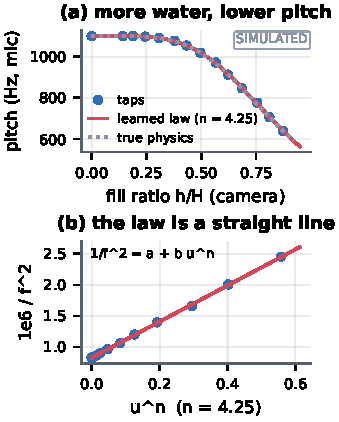
\includegraphics[width=\linewidth]{images/figures/fig_law_tall.pdf}
    \end{columns}
\end{frame}

% ------------------------------------------------------------------ learning from taps
\begin{frame}{Learning the law from taps: audio teaches vision}
    \label{sl:learning}
    \centering
    \resizebox{\linewidth}{!}{%
    \begin{tikzpicture}[font=\scriptsize, >={Stealth[length=2mm]}, node distance=5mm]
        \node[stage=gray] (tap) {\textbf{Tap}\\a bowl};
        \node[stage=gray, right=of tap] (meas) {\textcolor{camc}{camera: fill $r$}\\\textcolor{micc}{mic: pitch $f$}};
        \node[stage=phyc, right=of meas] (pt) {\textbf{one point}\\$(r, f)$};
        \node[stage=phyc, right=of pt] (fit) {\textbf{update}\\the line};
        \node[stage=fusc, right=of fit] (pred) {\textbf{camera alone}\\predicts pitch};
        \draw[->] (tap) -- (meas); \draw[->] (meas) -- (pt); \draw[->] (pt) -- (fit); \draw[->] (fit) -- (pred);
        \draw[->, gray] (pred.south) -- ++(0,-0.35) -| node[pos=0.25, below, font=\tiny] {next tap} (tap.south);
    \end{tikzpicture}}
    \vspace{1mm}
    \begin{columns}[T]
    \column{0.55\textwidth}
        \scriptsize
        \begin{itemize}
            \item \textbf{Start from physics:} a rough guess for $f_0$ and $\beta$, with wide uncertainty.
            \item \textbf{Each tap adds one point}; Bayesian linear regression \cite{bishop2006pattern} updates the straight line
                  \emph{and} says how sure it is.
            \item \textbf{The data choose $n$:} the best-supported exponent is $n = \EthreeN$ (theory 4).
            \item \textbf{Assumed noise:} pitch $\pm 8$ cents per tap; water level $\pm 0.6\,\%$ of the bowl.
        \end{itemize}
        \vspace{1mm}
        \textbf{Result:} after 5 taps the camera alone predicts any bowl's pitch within \textbf{\EfiveFive\ cents} (right).
    \column{0.43\textwidth}
        \centering
        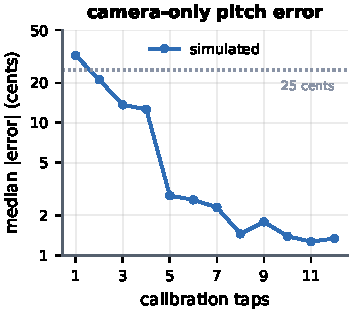
\includegraphics[width=\linewidth]{images/figures/fig_learning.pdf}
    \end{columns}
\end{frame}

% ------------------------------------------------------------------ fusion
\begin{frame}{Which bowl rang? Combining two clues}
    \label{sl:fusion}
    \begin{columns}[T]
    \column{0.54\textwidth}
        \scriptsize
        \begin{itemize}
            \item \textbf{Clue 1, sound:} the camera predicts each bowl's pitch from its water. The closer the heard pitch is
                  to a bowl's prediction, the higher that bowl scores (top right).
            \item \textbf{Clue 2, motion:} the striker tip lands on one bowl; nearby bowls score higher.
            \item \textbf{Combine:} multiply the two scores, trusting each clue by how reliable it is \emph{now}
                  \cite{ernst2002humans}: noisy sound $\Rightarrow$ trust motion; hidden striker $\Rightarrow$ trust sound.
            \item \textbf{Safety:} if no prediction fits the sound, the answer is ``none of these''.
        \end{itemize}
        \vspace{1mm}
        \textbf{Assumes} the two clues make independent errors (A7).
    \column{0.44\textwidth}
        \centering
        \resizebox{\linewidth}{!}{%
        \begin{tikzpicture}[font=\tiny, x=0.9cm, y=0.9cm]
            \draw[->] (0,0) -- (4.4,0) node[right] {pitch};
            \foreach \c/\lab in {0.6/1, 1.4/2, 2.2/3} {
                \pgfmathsetmacro{\lo}{\c-0.4}\pgfmathsetmacro{\hi}{\c+0.4}
                \draw[phyc, thick] plot[domain=\lo:\hi, samples=40] (\x,{0.9*exp(-((\x-\c)^2)/0.016)});
                \node[phyc] at (\c,1.02) {\lab};
            }
            \draw[phyc, thick] plot[domain=2.85:3.65, samples=40] (\x,{0.9*exp(-((\x-3.25)^2)/0.016)});
            \node[phyc, anchor=west] at (3.45,0.7) {4 and 5};
            \draw[micc, dashed, thick] (3.25,0) -- (3.25,1.05) node[above] {heard};
            \node at (2.1,-0.3) {predicted pitch of bowls 1--5 (from the camera)};
        \end{tikzpicture}}\\[2mm]
        \resizebox{\linewidth}{!}{%
        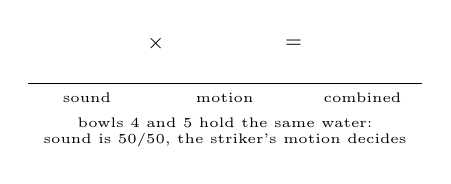
\begin{tikzpicture}[font=\scriptsize, x=1cm, y=1cm]
            \bars{0}{micc}{0.02}{0.02}{0.02}{0.47}{0.47}
            \bars{1.75}{camc}{0.02}{0.02}{0.03}{0.08}{0.85}
            \bars{3.5}{fusc}{0.0}{0.0}{0.0}{0.08}{0.92}
            \draw (-0.1,0) -- (4.9,0);
            \node at (1.52,0.5) {$\times$}; \node at (3.27,0.5) {$=$};
            \node[font=\tiny] at (0.645,-0.18) {sound}; \node[font=\tiny] at (2.395,-0.18) {motion}; \node[font=\tiny] at (4.145,-0.18) {combined};
            \node[font=\tiny, align=center] at (2.4,-0.62) {bowls 4 and 5 hold the same water:\\sound is 50/50, the striker's motion decides};
        \end{tikzpicture}}
    \end{columns}
\end{frame}

% ------------------------------------------------------------------ tuning
\begin{frame}{Tuning by sight: from a raga to millilitres}
    \label{sl:tuning}
    \begin{columns}[T]
    \column{0.53\textwidth}
        \scriptsize
        Raga Bhupali; each note is a fixed ratio of Sa:\\[1mm]
        \centerline{\begin{tabular}{@{}ccccc@{}}
            Sa & Re & Ga & Pa & Dha\\ \hline
            $1$ & $\tfrac98$ & $\tfrac54$ & $\tfrac32$ & $\tfrac53$
        \end{tabular}}
        \vspace{1mm}
        \begin{enumerate}
            \item \textbf{Pick Sa} so every note is reachable: water can only \emph{lower} a bowl's pitch.
            \item \textbf{Turn the law around:} note $\to$ water level $\to$ ml to pour (from the bowl's shape).
            \item \textbf{Stop one semitone early:} water is easy to add, hard to remove.
            \item \textbf{Tap once:} it shows how this bowl differs from the shared law; correct, then top up.
        \end{enumerate}
    \column{0.45\textwidth}
        \centering
        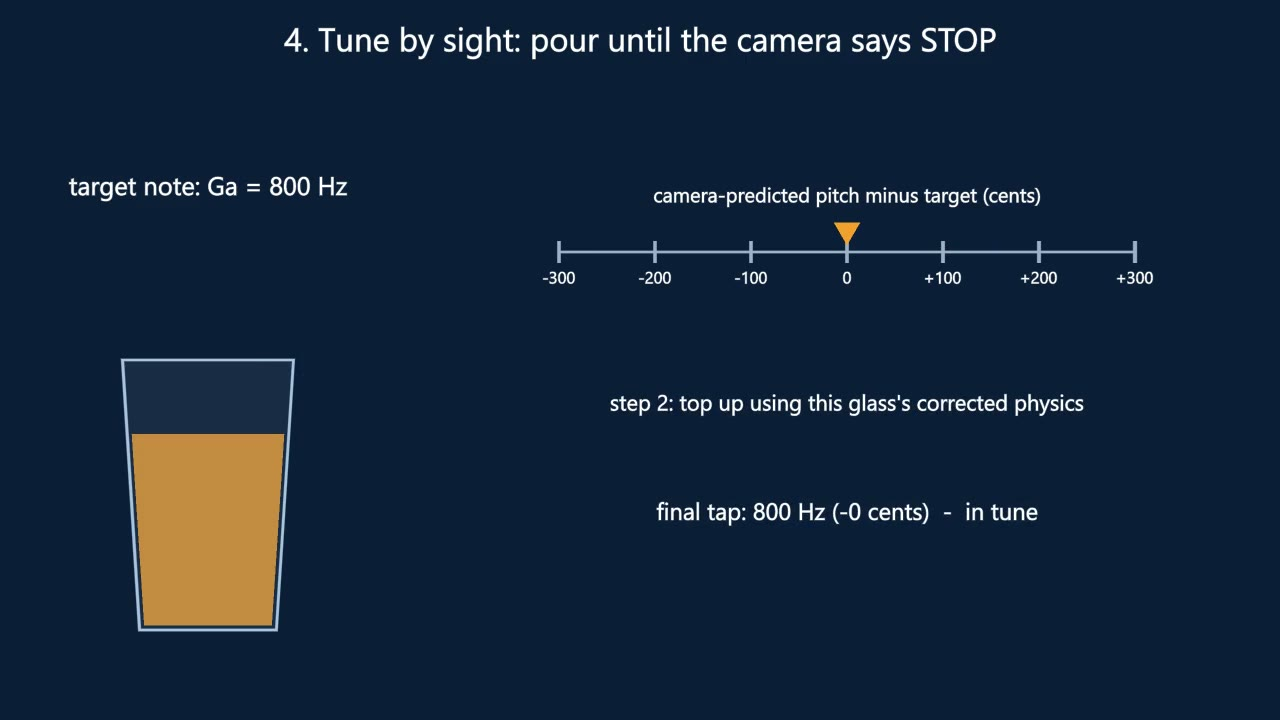
\includegraphics[width=\linewidth]{images/figures/anim_tune.jpg}\\[-0.5mm]
        {\tiny The camera's pitch gauge stops the pour; one tap fixes the last cents.\par}
    \end{columns}
    \vspace{2mm}
    \centering
    \resizebox{\linewidth}{!}{%
    \begin{tikzpicture}[font=\scriptsize, >={Stealth[length=2mm]}, node distance=4mm]
        \node[stage=camc] (plan) {\textbf{Plan}\\Sa, water levels};
        \node[stage=camc, right=of plan] (pour) {\textbf{Pour}\\camera tracks the level};
        \node[stage=phyc, right=of pour] (stop) {\textbf{Stop early}\\one semitone sharp};
        \node[stage=micc, right=of stop] (tap) {\textbf{Tap}\\measure the offset};
        \node[stage=camc, right=of tap] (top) {\textbf{Top up}\\corrected target};
        \node[stage=fusc, right=of top] (ok) {\textbf{Verify}\\tap: error in cents};
        \draw[->] (plan) -- (pour); \draw[->] (pour) -- (stop); \draw[->] (stop) -- (tap); \draw[->] (tap) -- (top); \draw[->] (top) -- (ok);
        \draw[->, gray] (ok.south) -- ++(0,-0.3) -| node[pos=0.25, below, font=\tiny] {next bowl} (pour.south);
    \end{tikzpicture}}
\end{frame}
